\documentclass[12pt,t,xcolor=dvipsnames]{beamer}
\usepackage{amsmath,amssymb}
\usepackage{multirow}
\usepackage{subfigure}
\usepackage{pgfplots}


% Beamer Commands
\setbeamertemplate{navigation symbols}{}
\setbeamertemplate{footline}
{%
\hspace*{0.7\linewidth}\insertshorttitle - p.\insertframenumber
}
\setbeamertemplate{footnote}
{%
\insertfootnotetext
}
\setbeamercolor{footnote mark}{fg=white}
\setbeamertemplate{frametitle}[default][center]
\setbeamertemplate{itemize item}[circle]
\setbeamertemplate{itemize subitem}[triangle]
\setbeamercolor{itemize subitem}{fg=Plum}
\setbeamerfont{itemize subitem}{size=\normalsize}
\setbeamercolor{alerted text}{fg=Magenta}
\setbeamerfont{institute}{size=\normalsize}
\setbeamerfont{list label}{series=\bfseries}
\usefonttheme[onlylarge]{structurebold} 

\newcommand{\alerta}[1]{{\usebeamercolor[fg]{frametitle} #1}}

% Title Page Stuff
\title{Final Report on the Black Arcs Problem}
\date{July 6, 2018}


\begin{document}

% Title Page
% - Begin Slide -----
\maketitle

% - Begin Slide -----
\begin{frame}
  \frametitle{Problem Summary}
  \onslide*<1>{
\vspace*{-12pt}
  \begin{center}
    Natural graphs of city layouts don't ``look nice''\\[12pt]

    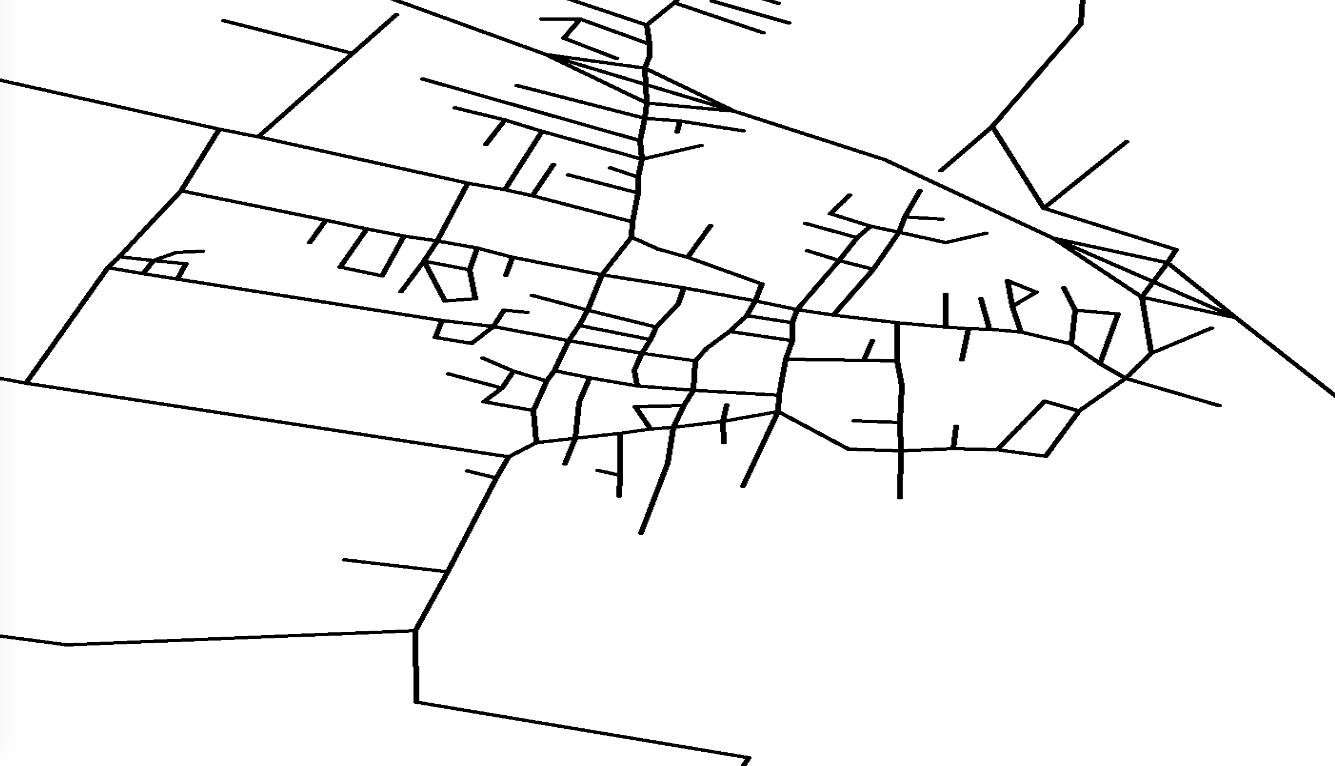
\includegraphics[width=\textwidth]{original_sackville}
  \end{center}}%
  \onslide*<2>{
    What does it mean to ``look nice''?
    \begin{itemize}
    \item Heuristic idea: sharp angles
    \item Ideal to have small set of allowable angles
    \item We take these to be multiples of $\pi/8$
	\item Want to encourage multiples of $\pi/2$ even more
    \end{itemize}

    Problem: how to translate graph nodes/edges to make angles more
    like multiples of $\pi/8$?
    }

\end{frame}

% - Begin Slide -----
\begin{frame}
  \frametitle{The Data}

  Get map data in list format:
  \begin{itemize}
  \item List of $n_v$ vertices as $(x_i,y_i)$ coordinates
  \item List of $n_e$ edges as vertex pairs
  \end{itemize}

  \begin{center}
    Look to translate nodes $(x_i,y_i) \rightarrow (\tilde{x}_i,\tilde{y}_i)$ so
    to ``improve'' angles formed by edges
  \end{center}
\pause
  Four principles:
  \begin{enumerate}
  \item Don't let nodes move a lot
  \item Don't let angles change a lot
  \item Make angles equal to $k\pi/8$ for some $k\in\mathbb{Z}$
  \item ``Encourage'' angles of $\pi/2$
  \end{enumerate}


\end{frame}


% - Begin Slide -----
\begin{frame}
  \frametitle{Continuous Optimization Approach}

  \begin{center}
    Central idea: relax constraint
  \end{center}

  Compose {\it fitness function} from three terms
  \begin{enumerate}
  \item Penalize node movement: $\displaystyle\sum_{i=1}^{n_v}
    \left((\tilde{x}_i-x_i)^2+(\tilde{y}_i - y_i)^2\right)$
  \item Penalize angle change: $\displaystyle\sum_{j=1}^{n_e} \left(\tilde{\theta}_j -
    \theta_j\right)^2$
    \begin{itemize}
    \item Given edge $e_j = \left\{(x_k,y_k),(x_\ell,y_\ell)\right\}$,
      define $\theta_j = \text{arctan2}(x_\ell-x_k,y_\ell-y_k)$
      %\item ``Four-quadrant inverse tangent''
    \end{itemize}
    \item Penalize difference from $k\pi/8$ and $\pi/2$ (again): $\displaystyle\sum_{j=1}^{n_e}\sin^2\left(8\tilde{\theta}_j\right)+\sin^2\left(2\tilde{\theta}_j\right)$
  \end{enumerate}
  
\end{frame}

% - Begin Slide -----
\begin{frame}
\frametitle{Fitness Function}

Take weighted sum of these:
\begin{align*}
f(\tilde{x},\tilde{y}) = \alpha&\sum_{i=1}^{n_v}
\left((\tilde{x}_i-x_i)^2+(\tilde{y}_i - y_i)^2\right)\\
& + \beta\sum_{j=1}^{n_e} \left(\tilde{\theta}_j - \theta_j\right)^2
+\gamma\sum_{j=1}^{n_e}\left(\sin^2(8\tilde{\theta}_j)+\sin^2(2\tilde{\theta}_j)\right)
\end{align*}

Problem: How to choose $\alpha$, $\beta$, $\gamma$?
\begin{itemize}
\item Eyeball it
\end{itemize}

\end{frame}

% - Begin Slide -----
\begin{frame}
  \frametitle{Black-Box Optimization Results}

  Many black-box optimization tools available
  \begin{itemize}
  \item Derivative-free optimization
    \begin{itemize}
    \item Powell seemed to provide better results than Nelder-Mead
    \end{itemize}
  \item Basin-hopping
    \begin{itemize}
    \item Very expensive
	\item Did not improve results enough visually to be used often
    \end{itemize}
  \item Differential Evolution
    \begin{itemize}
    \item Slower than Powell
    \end{itemize}
  \item CMA-ES
    \begin{itemize}
      \item DEAP (an evolutionary comptation framework for Python)
	  \item CMA-ES initial results were vastly different
    \end{itemize}
  \end{itemize}

\end{frame}

% - Begin Slide -----
\begin{frame}
  \frametitle{First results}
\begin{center}
  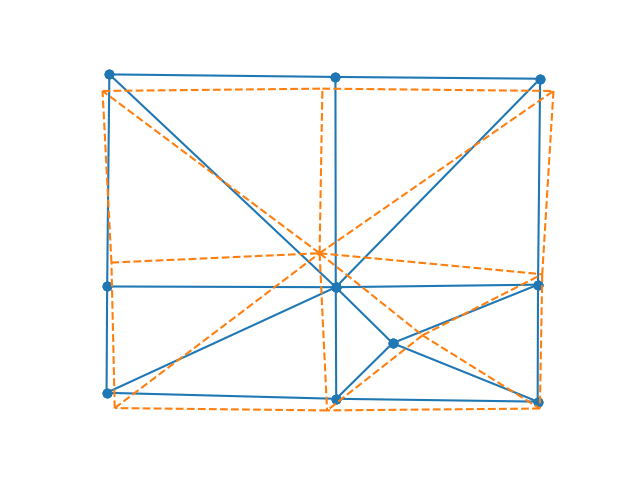
\includegraphics[width=\linewidth]{map1}
\end{center}
\end{frame}

% - Begin Slide -----
\begin{frame}
  \frametitle{Second results}
\begin{center}
  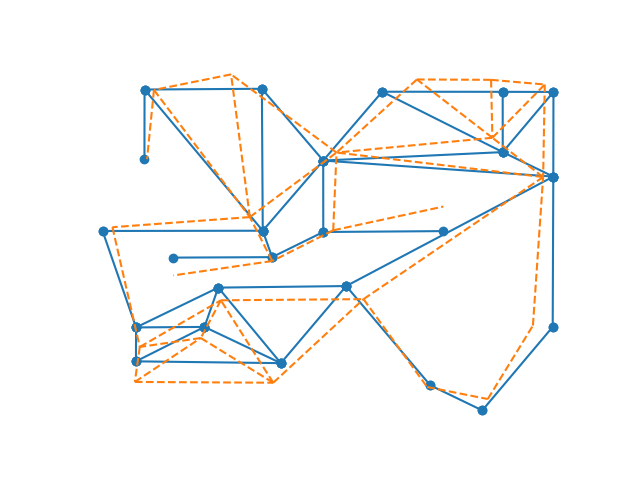
\includegraphics[width=\linewidth]{map2}
\end{center}
  

\end{frame}

% - Begin Slide -----
%\begin{frame}
%  \frametitle{Measuring Quality}
%
%  Visual quality seems good, but what about some numbers?
%  \onslide*<1>{
%  \begin{itemize}
%  \item For first example
%    \begin{itemize}
%    \item Reduce fitness function from 6.35 to 0.67
%    \item Reduce scaled deviation from angles of $k\pi/8$ from 0.45
%      to 0.10
%    \end{itemize}
%  \end{itemize}}%
%  \onslide*<2>{
%    \begin{itemize}
%    \item For second example
%      \begin{itemize}
%      \item Reduce fitness function from 21.29 to 1.61
%      \item Reduce scaled deviation from angles of $k\pi/8$ from 0.48
%        to 0.15
%      \end{itemize}
%    \end{itemize}
%
%  \begin{center}
%    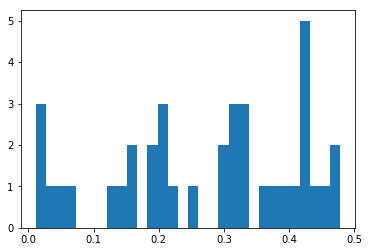
\includegraphics[width=0.48\linewidth]{../pngs/original_deviation_histogram}
%    \hspace*{0.01\linewidth}
%    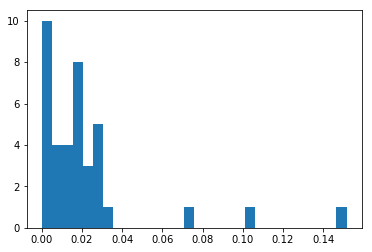
\includegraphics[width=0.48\linewidth]{../pngs/optimized_deviation_histogram}
%  \end{center}}%
%    
%        
%\end{frame}

% - Begin Slide -----
%\begin{frame}
%  \frametitle{Some choices}
%
%  \begin{center}
%    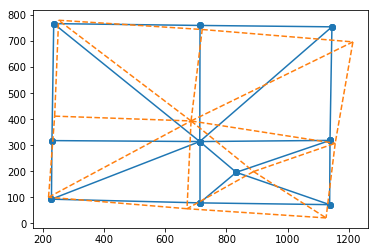
\includegraphics[width=0.48\linewidth]{../pngs/closer_terms}
%    \hspace*{0.01\linewidth}
%    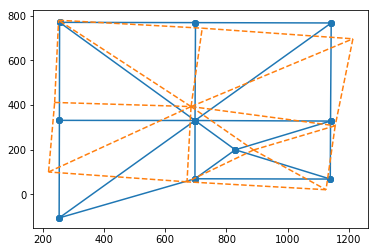
\includegraphics[width=0.48\linewidth]{../pngs/stuckout_term2}
%  \end{center}
%    
%  Two results from slightly different optimizer options
%  \begin{itemize}
%    \item Graph at right has much lower deviation in angles from
%      $k\pi/8$
%    \item Achieving lower deviation comes at trade-off with node displacement
%  \end{itemize}
%\end{frame}

% - Begin Slide -----
\begin{frame}
  \frametitle{Rotation}

  Idea: rotate first, then optimize relative to rotated map
  \begin{itemize}
  \item Eyeball $23^\circ$ rotation, from histogram of initial angles
    \begin{itemize}
    \item Did we automate this reliably? NO
    \end{itemize}
  \item Optimize after rotation
  \end{itemize}

\end{frame}

% - Begin Slide -----
\begin{frame}
  \frametitle{Results}

  \onslide*<1>{
    \begin{center}
      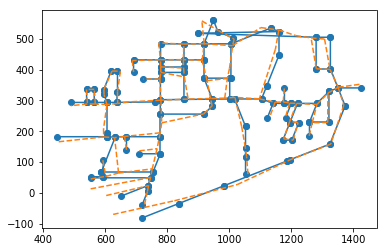
\includegraphics[width=\linewidth]{../pngs/map_6_powell}
    \end{center}
  }%
	\onslide*<2>{
    \begin{center}
      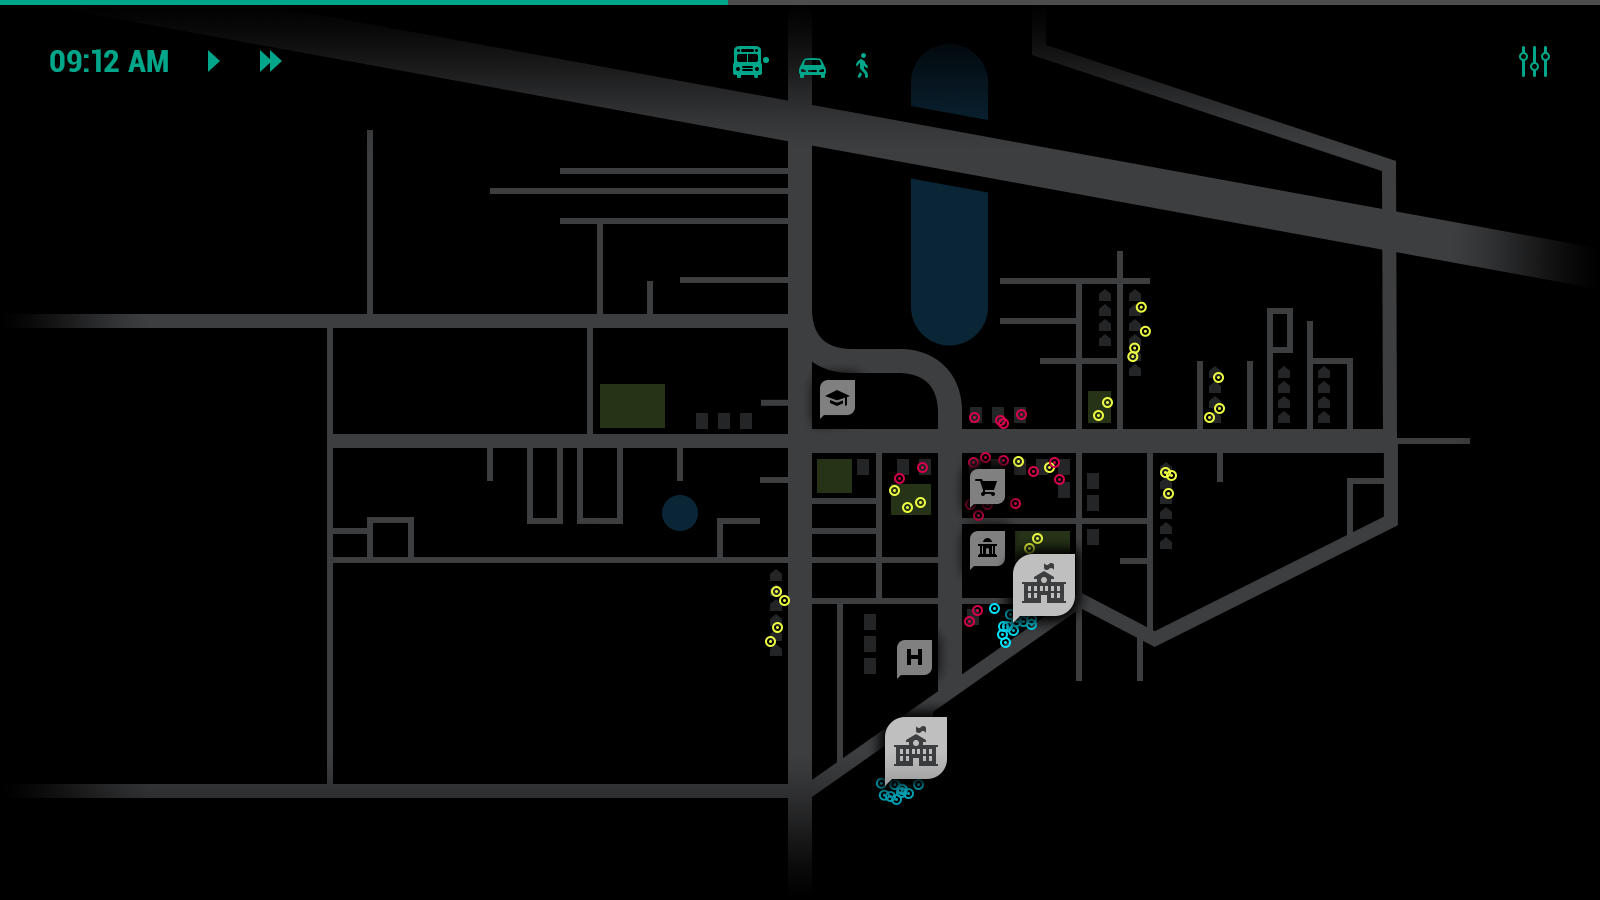
\includegraphics[width=\linewidth]{../pngs/artist_stylization}
    \end{center}
  }%

  

\end{frame}

\end{document}

% - Begin Slide -----
\begin{frame}
\frametitle{}

\end{frame}

% - Begin Slide -----
\begin{frame}
\frametitle{}

\end{frame}
